\documentclass[12pt]{article}
\usepackage[utf8]{inputenc}
\usepackage{multicol}
\usepackage{graphicx}
\usepackage{amsmath}
\usepackage{amsfonts}
\usepackage{mathtools}
\usepackage{siunitx}
\usepackage{braket}
\usepackage{parskip}
\usepackage{wrapfig}
\usepackage{xparse,mathtools}

\usepackage[letterpaper, portrait, margin=1in]{geometry}
\renewcommand{\baselinestretch}{1.05}
\title{Quantum HW9}
\author{bellenchia}
\date{March 2019}
\begin{document}
\maketitle

\section*{30.) One Parameter Variation}
\textbf{30 a.)}
Let us demonstrate the Variation of Parameters technique on a system we're already familiar with, where our potential is that of the Harmonic Oscillator; $V(x)=\frac{m\omega^2x^2}{2}$\\
Given the trial function $\phi=e^{-\alpha x^2}$, we first calculate the inner product with itself. \\

Note that since our function is even ($ \phi(x)=\phi(-x) $) we know ${\displaystyle\int_{-\infty}^\infty}|\phi|^2x=2{\displaystyle\int_0^\infty}|\phi|^2 dx$\\

The integral of our Gaussian is $ {\displaystyle\int_0^\infty} e^{-2\alpha x^2 dx}=\sqrt{\frac{\pi}{2\alpha}}$, this is a classic result modified by our variable.\\

Computing our Hamiltonian, we find $\hat{H}\phi=\frac{1}{2}(x^2-(4\alpha^2x^2-2\alpha))e^{-\alpha x^2}$\\

Next, we find $\braket{\hat{H}}=\braket{\phi|\hat{H}|\phi}=2{\displaystyle\int_{0}^\infty}e^{-2\alpha x^2}\frac{1}{2}[(1-4\alpha^2)x^2+2\alpha]dx$\\

Evaluating this, we get $\sqrt{\frac{\pi}{2}}\frac{4\alpha^2+1}{8\alpha^{3/2}}$, so we reach $\frac{\braket{\phi|\hat{H}|\phi}}{\braket{\phi|\phi}}= \sqrt{\frac{\pi}{2}}\frac{4\alpha^2+1}{8\alpha^{3/2}} / \sqrt{\frac{\pi}{2\alpha}}=\frac{4\alpha^2+1}{8\alpha}=\frac{\alpha}{2}+\frac{1}{8\alpha}$\\

$\Rightarrow\frac{\braket{\phi|\hat{H}|\phi}}{\braket{\phi|\phi}}=\frac{\alpha}{2}+\frac{1}{8\alpha}$, we want to find the value of $\alpha$ to minimize our result; $\frac{\alpha}{2}+\frac{1}{8\alpha}\geq E_{\text{ground}}$\\

We know the ground state energy of the Harmonic Oscillator is $E_{\text{ground}}=\frac{\hbar\omega}{2}$, or in our units just simply $\frac12$. Without any algebra it is clear $\alpha=\frac{1}{2}\Rightarrow E_{\text{ground}}=\frac{1}{2}$\\

To be precise, we could set our result equal to one half, then multiply each side by $\alpha$ then set up an equation of the form $c_0+c_1\alpha+c_2\alpha^2=0$, and solve using the quadratic formula. This is the method we used for the next part.\\

\textbf{30 b.)}\\

With our new trial function, $\phi=\text{sech}^2(x)$, we calculate the necessary integrals;\\

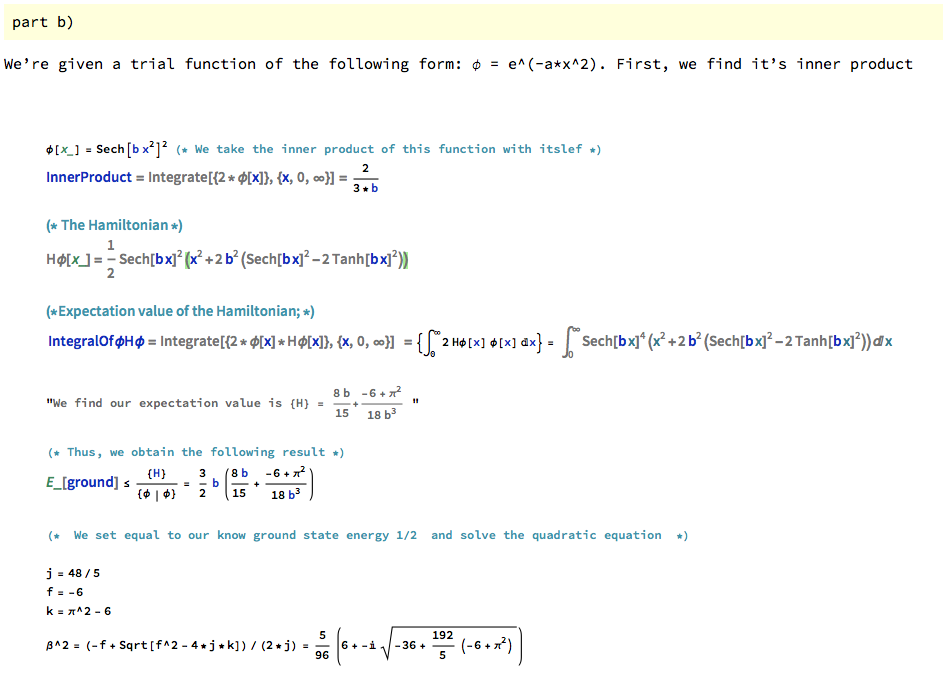
\includegraphics[width=\linewidth]{blart6.png}

It appears we have found that $\frac{\braket{\phi|\hat{H}|\phi}}{\braket{\phi|\phi}}=\frac{3\beta}{2}(\frac{4\beta}{15}+\frac{\pi^2-6}{36\beta^3})=\frac{2\beta^2}{5}+\frac{\pi^2-6}{12\beta^3}$. Let us find the parameter value such that we get our desired energy of $E_{\text{ground}}=\frac12$\\

$(\frac{2\beta^2}{5}+\frac{\pi^2-6}{24\beta^2})=\frac12$, multiplying both sides by $ 24\beta^2 $; $ (\frac{48}{5})\beta^4-(12)\beta^2+(\pi^2-6)=0 $\\

Using the quadratic formula, we obtain $\beta^2=\frac{5}{96}(12\pm\sqrt{144-\frac{192}{5}(\pi^2-6)})$\\

Thus, our final values are $\beta=\pm\sqrt{\frac{5}{96}(12\pm\sqrt{144-\frac{192}{5}(\pi^2-6)})}$\\

Since $\text{Sech}(x)^2=\text{Sech}(-x)^2$, the latter twofold degeneracy is irrelevant. Meaning we have two values, each of the form $\beta_1=a_1+ib_1$ and $\beta_2=a_1-ib_1$. This degeneracy doesn't reflect on the final function, shown in the former of the two following graphs, where both $\phi_{\beta1}$ and $\phi_{\beta2}$ are plotted atop one another.\\

The second plot shows the trial function plotted along with the actual, gaussian solution to the ground state of the Harmonic Oscillator problem.

\begin{figure}[h!]
    \centering
    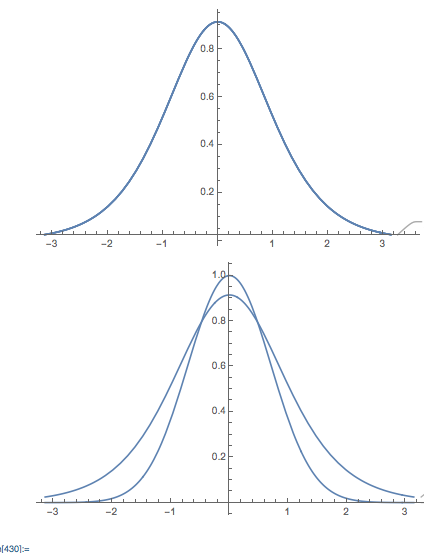
\includegraphics[width=0.8\linewidth]{111.png}
\end{figure}

\section*{31.) Time Evolution Operator}

We have $\hat{U}(t,t_0)=exp(-i\hat{H}(t-t_0)/\hbar)$ which written as a summation is;\\

$\hat{U}(t,t_0)={\sum_{n=0}^\infty}\frac{1}{n!}(-i(t-t_0)/\hbar)^n\hat{H}^n$\\

\textbf{a)} Now, taking $\hat{U}\ket{\Psi(x,t_0)}$, and acknowledging that \textit{by the Schrodinger equation}; $\hat{H}\ket{\Psi}=i\hbar\frac{d}{dt}\ket{\Psi}$\\

$\hat{U}\ket{\Psi(x,t_0)}=\sum_{0}^\infty[\frac{1}{n!}(\frac{-i(t-t_0)}{\hbar})^n(i\hbar)^n\frac{d^n}{dt^n}\ket{\Psi}]$\\

This is clearly the form of the \textbf{Taylor Expansion} of $\ket{\Psi(x,t)}$ about $t=t_0$. Thus, we can write $\hat{U}\ket{\Psi(x,t_0)}=\ket{\Psi(x,t)}$\\

\textbf{b) } To show this operator satisfies $\hat{U}^\dagger\hat{U}=1$ we must understand that $\hat{H}$ is a Hermitian operator, and therefore is equal to its conjugate transpose, $\hat{H}^\dagger=\hat{H}$\\

$\Rightarrow\hat{U}^\dagger=exp(\frac{i(t-t_0)\hat{H}}{\hbar})$, and it is simple to find;\\

$\hat{U}^\dagger\hat{U}=exp(\frac{-i(t-t_0)\hat{H}}{\hbar})exp(\frac{i(t-t_0)\hat{H}}{\hbar})=1$\\

\section{32.) Quantum Diffusion Monte Carlo}

Now, we are taking a trial function allowed to vary over \textit{imaginary time};  $\ket{\phi_\tau}=exp(-\tau\hat{H}t/\hbar)\ket{\phi}$\\

Since the Hamiltonian commuted with all functions of itself; $\hat{H}\ket{\phi_\tau}=\sum_0^\infty(-\tau/\hbar)^n\frac{1}{n!}\hat{H}^{n+1}$\\

We rewrite this again using $\hat{H}=i\hbar\frac{d}{dt}$ so we have $\hat{H}\ket{\phi_\tau}=\sum_0^\infty(-\tau/\hbar)^n\frac{1}{n!}(i\hbar)^{n+1}\frac{d^{n+1}}{dt^{n+1}}\ket{\phi}$\\


Next, we can take the product of our two series; $\braket{\phi_\tau|\hat{H}|\phi_\tau}=exp(-\tau\hat{H}t/\hbar)\ket{\phi}*\sum_0^\infty(-\tau/\hbar)^n\frac{1}{n!}\hat{H}^{n+1}$\\

$\braket{\phi_\tau|\hat{H}|\phi_\tau}=\sum_0^\infty(-\tau/\hbar)^{2n}(\frac{1}{n!})^2\hat{H}^{2n+1}\ket{\phi}$

The norm of this trial function also changes, $\braket{\phi_\tau|\phi_\tau}={\displaystyle\int}[e^{-2\tau\hat{H}/\hbar}\psi(\vec{r})]d^3\vec{r}$\\

\textbf{Wait, disregard that}

That may have been the wrong way to go about things... here's another method;

Now, we know $\frac{d}{dt}\ket{\phi_\tau}=(-\tau/\hbar)\ket{\phi_\tau}$\\

So therefore, $\hat{H}\ket{\phi_\tau}=(i\hbar)(-\tau/\hbar)=-i\tau$\\

Thus, $\braket{\phi_\tau|\hat{H}|\phi_\tau}=\braket{\phi_tau|(-i\tau)|\phi_tau}=-i\tau\braket{\phi_\tau|\phi_\tau}$\\

So our expectation value is $\frac{\braket{\phi_\tau|\hat{H}|\phi_\tau}}{\braket{\phi_tau|\phi_\tau}}=-i\tau$\\

\end{document}
